\documentclass[english,14pt]{beamer}
\usetheme{EastLansing}
\usecolortheme{spruce}

\usepackage{xcolor}
\usepackage{listings}
\usepackage{courier}
\usepackage{graphicx}
\usepackage{amsmath}
\usepackage{algorithm2e}
\usepackage{multicol}
\usepackage{hyperref}
\usepackage{textcomp}

% http://mirrors.ibiblio.org/CTAN/macros/latex/contrib/datetime2/datetime2.pdf
\usepackage{babel}
\usepackage[useregional]{datetime2}

% https://tex.stackexchange.com/questions/42619/x-mark-to-match-checkmark
\usepackage{pifont}% http://ctan.org/pkg/pifont

%% https://stackoverflow.com/questions/1435837/how-to-remove-footers-of-latex-beamer-templates
%%gets rid of bottom navigation bars
%\setbeamertemplate{footline}[page number]
%
%gets rid of navigation symbols
\setbeamertemplate{navigation symbols}{}


\usefonttheme[onlymath]{serif}

\definecolor{mGreen}{rgb}{0,0.6,0}
\definecolor{mGray}{rgb}{0.5,0.5,0.5}
\definecolor{mPurple}{rgb}{0.8,0,0.82}
\definecolor{backgroundColour}{rgb}{0.95,0.95,0.92}
\definecolor{lightBlue}{rgb}{0.1, 0.1, 0.8}

\newcommand\red[1]{{\color{red} #1}}
\newcommand\green[1]{{\color{green} #1}}
\newcommand\blue[1]{{\color{blue} #1}}

\newcommand{\cmark}{\ding{51}}%
\newcommand{\xmark}{\ding{55}}%

\lstdefinestyle{CStyle}{
    backgroundcolor=\color{backgroundColour},   
    commentstyle=\color{mGreen},
    keywordstyle=\color{magenta},
    numberstyle=\tiny\color{mGray},
    stringstyle=\color{mPurple},
    basicstyle=\footnotesize,
    breakatwhitespace=false,         
    breaklines=true,                 
    captionpos=b,                    
    keepspaces=true,                 
    numbers=left,                    
    numbersep=5pt,                  
    showspaces=false,                
    showstringspaces=false,
    showtabs=false,                  
    tabsize=2,
    language=Python
}

\lstdefinestyle{pseudo}{
        basicstyle=\ttfamily\footnotesize,
        keywordstyle=\color{lightBlue},
        morekeywords={BEGIN,END,IF,ELSE,ENDIF,ELSEIF,PRINT,WHILE,RETURN,ENDWHILE,DO,FOR,TO,IN,ENDFOR,BREAK,INPUT},
        morecomment=[l]{//},
        commentstyle=\color{mGreen}
}

\lstset{basicstyle=\footnotesize\ttfamily,breaklines=true}
\lstset{framextopmargin=50pt,tabsize=2}

\title{ENGG1003 - Thursday Week 4}
\subtitle{Using random numbers, and reading from spreadsheets}
\author{Steve Weller \& Sarah Johnson}
\institute{University of Newcastle}
%\date{\today}
\date{18 March, 2021}

% following is a bit of a hack, but forces page numbers (technically: frame numbers) to run 1,2,3,... 
% with titlepage counting as frame 1

\addtocounter{framenumber}{1}
\titlepage

\begin{document}

\begin{flushleft}
{\scriptsize Last compiled:~\DTMnow}
\vspace*{-5mm}
\end{flushleft}
\framebreak

%==============================================================

\begin{frame}[fragile]

\frametitle{Lecture overview}
\begin{enumerate}
	\item Using random numbers


	\item[]
	
	\item Reading from spreadsheets

	\item[]
\end{enumerate}

\begin{itemize}
	\item More practice with arrays, iteration, \\ conditional code execution (\texttt{if}) and plotting
\end{itemize}

\end{frame}

%==============================================================

\begin{frame}[fragile]

\frametitle{$1)$ Using random numbers}

\textbf{Recap:~} generating random numbers

\begin{figure}[ht]
	\centering
	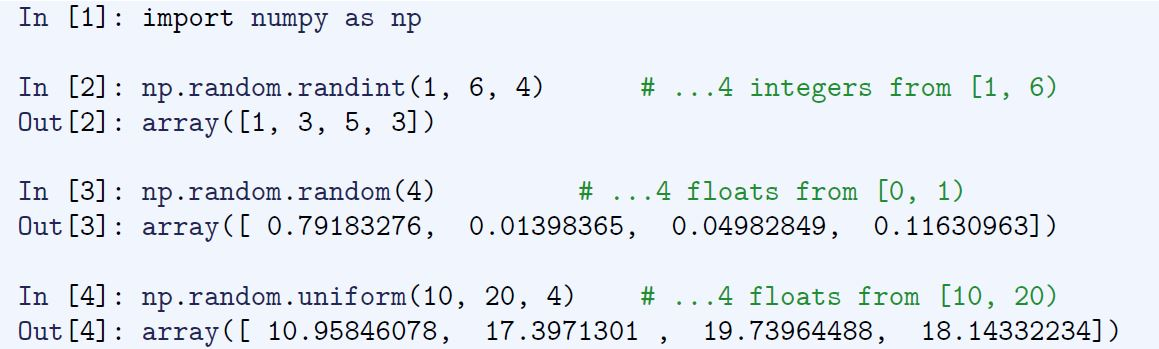
\includegraphics[width=\textwidth]{figures/LLp55b}
\end{figure}
\vspace*{-3mm}
Using \texttt{numpy} library:
\begin{itemize}
	\item random integers
	\item random floats from $[0,1)$
	\item random floats from $[a,b]$
\end{itemize}

\end{frame}

%==============================================================

\begin{frame}[fragile]

\frametitle{Random integers: simulating coin toss}

\textbf{Example 1}\\
\vspace*{5mm}

Simulate the toss of a coin $N$ times as follows:

\begin{itemize}
	\item generate a length-$N$ array of randomly chosen $0$s and $1$s
	\begin{itemize}
		\item $0 = $~heads, $1 = $~tails
		\item equally likely heads and tails ie: fair coin
	\end{itemize}
	\item[]
	\item display \emph{expected} number of heads observed
	\item display \emph{actual} number of heads observed
	\item test/debug with $N=100$, then $N=100,000$
\end{itemize}

\end{frame}

%==============================================================

\begin{frame}[fragile]

\frametitle{Coin toss simulation}
\vspace*{-3mm}
\begin{lstlisting}[style=CStyle]
import numpy as np

# generate random array of 0s and 1s
# 0==heads & 1==tails
# N integers from [0,2) ie: 0 or 1
N = 100000
x = np.random.randint(0, 2, N)
print(x)

headCnt = 0;
for i in range(0,N,1):
    if x[i]==0:
        headCnt += 1

print('Expected number of heads: {}'.format(N/2))
print('Observed number of heads: {}'.format(headCnt))
\end{lstlisting}
\vspace*{-3mm}
\begin{itemize}
	\item Live demo of \texttt{headsTails.py}
\end{itemize}

\end{frame}

%==============================================================

\begin{frame}[fragile]

\frametitle{Random floats: engineering tolerance}

\textbf{Example 2}\\
\vspace*{2mm}
\begin{itemize}
	\item steel bolts manufactured with length uniformly distributed between $17~$mm and $19$~mm
	\item only bolts with length in range $[17.25,18.75]$~mm are within tolerance ie: acceptable
	\item write Python code with random numbers to estimate percentage of bolts which are acceptable
	\begin{itemize}
		\item demonstrate your code for $N=10,000$
		\item compare with expected percentage of acceptable bolts:
		\[
			100 \times \frac{18.75-17.25}{19-17} = 75\%
		\]
	\end{itemize}
\end{itemize}

\end{frame}

%==============================================================

\begin{frame}[fragile]

\frametitle{Engineering tolerance simulation}
\vspace*{-3mm}
\begin{lstlisting}[style=CStyle]
import numpy as np

# generate random array of N floats in range [17,19]
N = 10000
x = np.random.uniform(17,19,N)
tolLow = 17.25
tolHigh = 18.75
#print(x)

goodCnt = 0;
for i in range(0,N,1):
    if tolLow <= x[i] <= tolHigh:
        goodCnt += 1

print('Percentage of parts within tolerance: {}%'.format(100*goodCnt/N))
\end{lstlisting}
\vspace*{-3mm}
\begin{itemize}
	\item Live demo of \texttt{engTolerance.py}
\end{itemize}
\end{frame}

%==============================================================

\begin{frame}[fragile]

\frametitle{Random floats: simulate dartboard}

\textbf{Example 3}\\
\vspace*{1mm}
\begin{itemize}
	\item a circular dartboard radius $1$~m is centred in the middle of a square, side length $2$~m
	\item darts are thrown randomly and land with uniform probability in the square
	\begin{itemize}
		\item most (but not all) darts land inside the circle
	\end{itemize}
	\pause
	\item write a Python program which puts a \red{red} dot if the dart lands inside (or on the perimeter) of the circle, and a \blue{blue} dot otherwise
	\begin{itemize}
		\item Hint: points inside (or on perimeter) of circle satisfy
			\[
			x^2 + y^2 \leq 1
			\]
		\end{itemize}
	\item run your program with $N=100, 1000$ and $10,000$
\end{itemize}

\end{frame}

%==============================================================

\begin{frame}[fragile]

\frametitle{Dartboard simulation: code}
\begin{lstlisting}[style=CStyle,basicstyle=\scriptsize]
import numpy as np
import matplotlib.pyplot as plt

# generate random array of (x,y) pairs covering
# square with edge length 2
N = 10000
x = np.random.uniform(-1, 1, N)   # N floats from [-1,1]
y = np.random.uniform(-1, 1, N)   # N floats from [-1,1]

insideCnt = 0;
for i in range(0,N,1):
    if x[i]**2 + y[i]**2 <= 1:
        plt.plot(x[i],y[i],'r.')
    else:
        plt.plot(x[i],y[i],'b.')

plt.axis('equal')   # plot with aspect ratio 1:1
plt.show()
\end{lstlisting}
\vspace*{-3mm}
\begin{itemize}
	\item Live demo of \texttt{dartboard.py}
\end{itemize}
\end{frame}

%==============================================================

\begin{frame}[fragile]

\frametitle{Dartboard simulation: output}

\begin{itemize}
	\item two length-$N$ arrays of random numbers
	\begin{itemize}
		\item \texttt{x = [x[0],x[1],...,x[N-1]]}
		\item \texttt{y = [y[0],y[1],...,y[N-1]]}
	\end{itemize}
	\item \texttt{x[i]} $\in [-1,+1]$ for all $i$, similar for \texttt{y[i]}
	\item position $(x_i,y_i)$ of $i$-th dart is (\texttt{x[i],y[i]})
\end{itemize}

\begin{figure}[ht]
	\centering
	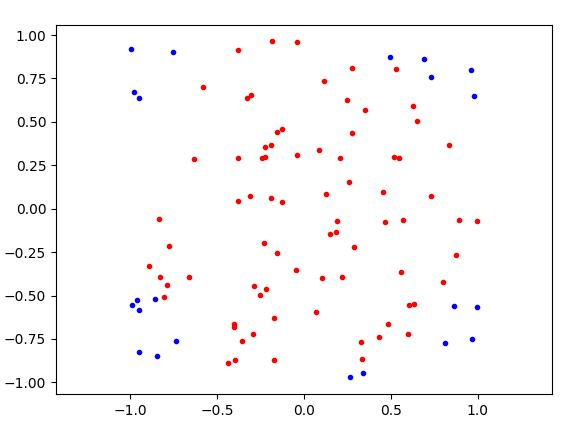
\includegraphics[width=0.33\textwidth]{figures/dartboard100}%
	\pause
	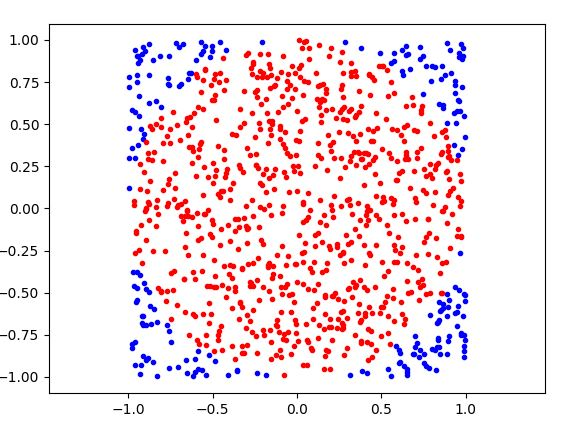
\includegraphics[width=0.33\textwidth]{figures/dartboard1000}%
	\pause
	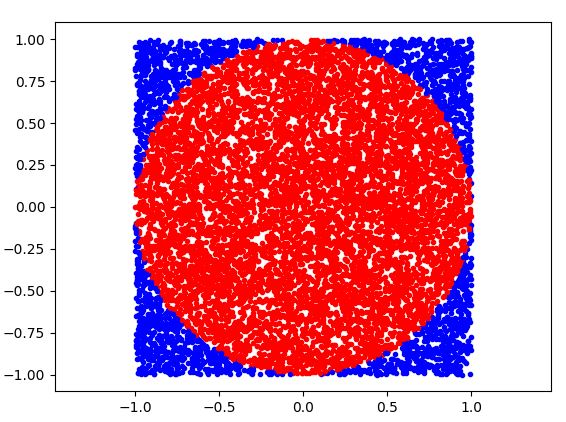
\includegraphics[width=0.33\textwidth]{figures/dartboard10000}
\end{figure}

\end{frame}

%==============================================================

\begin{frame}[fragile]

\frametitle{Random floats: estimate $\pi$}

\textbf{Example 4}\\
\begin{itemize}
	\item modify Example~3 to count number of points inside (or on) circle
	\item use your results to estimate the value of $\pi$
	\pause
	\item strategy:
	\begin{itemize}
		\item area of square: $2 \times 2 = 4$
		\item area of circle: $\pi r^2$, where radius $r=1$, hence area is $\pi$
		\item[]
		\[
			R = \frac{\mathrm{area~of~circle}}{\mathrm{area~of~square}} = \frac{\pi}{4}
		\]
		\pause		
		\begin{eqnarray*}
			\mathrm{estimate~of~} \pi & = & 4\times \mathrm{estimate~of~ratio~} R \\
			& =& 4 \times \frac{\mathrm{number~of~points~in~circle}}{\mathrm{total~number~of~points}}
		\end{eqnarray*}
	\end{itemize}
\end{itemize}

\end{frame}

%==============================================================

\begin{frame}[fragile]

\frametitle{Estimate $\pi$: code}
\vspace*{-5mm}
\begin{lstlisting}[style=CStyle,basicstyle=\scriptsize]
import numpy as np
import matplotlib.pyplot as plt

# generate random array of (x,y) pairs covering
# square with edge length 2
N = 10000
x = np.random.uniform(-1, 1, N)      # N floats from [-1,1]
y = np.random.uniform(-1, 1, N)      # N floats from [-1,1]

insideCnt = 0;
for i in range(0,N,1):
    if x[i]**2 + y[i]**2 <= 1:
        plt.plot(x[i],y[i],'r.')
        insideCnt += 1
    else:
        plt.plot(x[i],y[i],'b.')

R = insideCnt/N
print('Estimate of pi: {}'.format(4*R))

plt.axis('equal')
plt.show()
\end{lstlisting}
\vspace*{-3mm}
\begin{itemize}
	\item Live demo of \texttt{estimatePi.py}
\end{itemize}
\end{frame}

%==============================================================

\begin{frame}[fragile]

\frametitle{$2)$ Reading from spreadsheets}

\begin{itemize}
    \item so far have been working ``toy problems'' with small data sets
    \item engineers and scientists often work with \emph{large} datasets
        \begin{itemize}
            \item spreadsheets eg: CSV or XML files
            \item databases eg: SQL files 
            \item wide range of other software packages
        \end{itemize}
    \item there's a package for that:~it's called \texttt{pandas}
    \item[] \ldots and we can import it just like \texttt{numpy} and \texttt{matplotlib}
\begin{lstlisting}[style=CStyle]
import pandas as pd
\end{lstlisting}
\end{itemize}

\end{frame}

%==============================================================

\begin{frame}[fragile]

\frametitle{Data import using pandas}
\begin{itemize}
    
    \item to import data from \red{\emph{comma-separated values}} (CSV) file into Python:
\begin{lstlisting}[style=CStyle]
import pandas as pd
mydata = pd.read_csv('filename.csv')
\end{lstlisting}

	\item[]

	\item if CSV file is not in the same folder as Python project, need to specify its location with a path:
\begin{lstlisting}[style=CStyle]
import pandas as pd
mydata = pd.read_csv('c:\Myfolder\filename.csv')
\end{lstlisting}
\end{itemize}

\end{frame}

%==============================================================

\begin{frame}[fragile]

\frametitle{Checking data import}

\begin{itemize}
	\item \texttt{pandas} imports contents of spreadsheet into something called a \red{\emph{data structure}}
	
	\begin{itemize}
	    \item we won't spend any time on today but may get back to later in the course
	\end{itemize}
	\item[]
	\item To check data imported into \texttt{mydata} the following instruction is very useful:
\begin{lstlisting}[style=CStyle]
print(mydata.head())
\end{lstlisting}
	\item[]
	\item This prints out the first few lines of the data set
\end{itemize}

\end{frame}

%==============================================================

\begin{frame}[fragile]

\frametitle{Extracting data into an array}

\begin{itemize}
	\item One final very useful instruction will extract a column of the data and save it as a \texttt{numpy} array
	\begin{itemize}
		\item uses the column name in the original spreadsheet
	\end{itemize}
	
	\item[]
	
\begin{lstlisting}[style=CStyle]
mycolumn = mydata['column_name'].values   
\end{lstlisting}
	\item[]
	\item We can now process this data using the Python skills we have been building in this course
\end{itemize}

\end{frame}

%==============================================================

\begin{frame}[fragile]
\frametitle{Example}
\begin{itemize}
    \item We have a CSV spreadsheet (\texttt{Rainfall.csv}) which records annual rainfall for 20 regions over the last 10 years
    \begin{figure} 
        \centering
        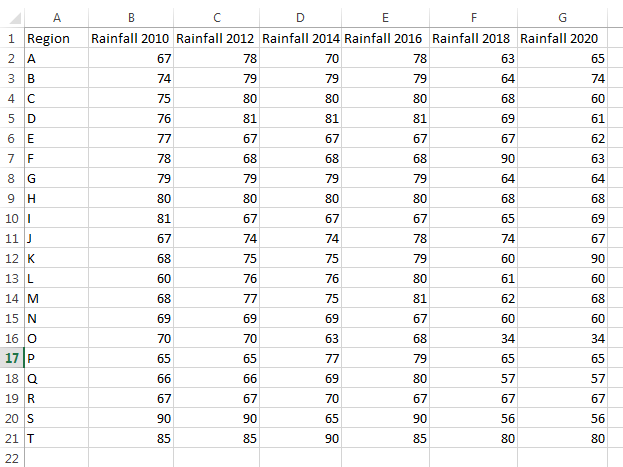
\includegraphics[width=5cm]{figures/excel_rainfall.PNG}
        \label{fig:my_label}
    \end{figure}
    \item We would like to know how many regions have seen a reduction in rainfall between 2010 and 2020
\end{itemize}
\end{frame}

%==============================================================

\begin{frame}[fragile]
\frametitle{Example}
\begin{lstlisting}[style=CStyle]
import pandas as pd

# import the rainfall data 
Rainfalldata = pd.read_csv("Rainfall.csv")
print(Rainfalldata.head())

# extract the columns for 2010 and 2020 
Rainfall2010 = Rainfalldata['Rainfall 2010'].values         
Rainfall2020 = Rainfalldata['Rainfall 2020'].values         

\end{lstlisting}
\end{frame}

%==============================================================

\begin{frame}[fragile]
\frametitle{Example}
\begin{lstlisting}[style=CStyle]
# How many regions have seen a decrease in rainfall 
N = len(Rainfall2010)
count = 0
for i in range(0, N, 1):
    if Rainfall2020[i] < Rainfall2010[i]:
        count = count + 1

percentage_decreased = count/N*100

print('Of the {} regions, {} have reduced rainfall which is {:f6.2}% '.format(N, count, percentage_decreased))
\end{lstlisting}
\end{frame}

%==============================================================

\begin{frame}[fragile]

\frametitle{Lecture summary}
\begin{enumerate}
	\item Using random numbers
	\item[]
	
	\item Reading from spreadsheets
\end{enumerate}

\begin{itemize}
	\item[]
	\item \textbf{Next lecture:~} functions in Python, Chapter 4 \\ of LL textbook
\end{itemize}

\end{frame}

\end{document}